\subsection{Критерии интегрируемости ограниченной на отрезке функции}

Рассматривается вопрос о необходимых и достаточных условиях того, что функция $f(x)$ является интегрируемой по Риману на отрезке $[a, b]$. Лектор отмечает, что поскольку интегрируемость по Риману влечет за собой ограниченность функции, критерии формулируются для класса ограниченных функций.

Основным инструментом здесь выступает связь между интегральными суммами Римана и суммами Дарбу.

\begin{theorem}[Критерий Дарбу]
Ограниченная на отрезке $[a, b]$ функция $f(x)$ интегрируема по Риману на этом отрезке тогда и только тогда, когда предел разности верхней и нижней сумм Дарбу при стремлении диаметра разбиения к нулю равен нулю:
\[ \lim_{\lambda(P) \to 0} (S(P) - s(P)) = 0 \]
\end{theorem}

\begin{tcolorbox}[title=Доказательство, breakable]
Доказательство состоит из обоснования необходимости и достаточности.

\textbf{1. Необходимость ($\implies$):}
Пусть функция $f(x)$ интегрируема на $[a, b]$. Это означает, что существует число $I$ (интеграл), такое что для любого $\eps > 0$ существует $\delta > 0$, при котором для любого разбиения $P$ с диаметром $\lambda(P) < \delta$ и любого набора отмеченных точек $\xi$:
\[ | \sigma(f, P, \xi) - I | < \eps \]
Раскрывая модуль, получаем:
\[ I - \eps < \sigma(f, P, \xi) < I + \eps \]
Это неравенство справедливо для \textit{любого} набора $\xi$ при фиксированном разбиении $P$. Поскольку нижняя сумма Дарбу $s(P)$ является точной нижней гранью интегральных сумм по всем наборам $\xi$, а верхняя сумма $S(P)$ — точной верхней гранью, при переходе к граням неравенства сохраняются:
\[ I - \eps \le s(P) \le S(P) \le I + \eps \]
Отсюда следует, что разность сумм Дарбу:
\[ S(P) - s(P) \le (I + \eps) - (I - \eps) = 2\eps \]
Так как $\eps$ произвольно, это означает, что $\lim_{\lambda(P) \to 0} (S(P) - s(P)) = 0$.

\textbf{2. Достаточность ($\impliedby$):}
Пусть $\lim_{\lambda(P) \to 0} (S(P) - s(P)) = 0$. 
Сначала заметим, что для любых разбиений выполняется неравенство для интегралов Дарбу: $\underline{I} \le \overline{I}$. Кроме того, для любого фиксированного разбиения $P$ всегда:
\[ s(P) \le \underline{I} \le \overline{I} \le S(P) \]
Следовательно:
\[ 0 \le \overline{I} - \underline{I} \le S(P) - s(P) \]
Так как правая часть стремится к нулю при $\lambda(P) \to 0$, а числа $\overline{I}$ и $\underline{I}$ не зависят от разбиения, то $\overline{I} - \underline{I} = 0$, то есть $\underline{I} = \overline{I} = I$.
Теперь рассмотрим произвольную интегральную сумму $\sigma(f, P, \xi)$. По свойствам сумм Дарбу:
\[ s(P) \le \sigma(f, P, \xi) \le S(P) \]
Поскольку и $s(P)$, и $S(P)$ при $\lambda(P) \to 0$ стремятся к одному и тому же числу $I$, то по теореме о зажатой функции:
\[ \lim_{\lambda(P) \to 0} \sigma(f, P, \xi) = I \]
Это по определению означает, что функция $f(x)$ интегрируема по Риману.
\end{tcolorbox}

\subsubsection*{Критерий в терминах колебаний}

Для практического применения часто используется переформулировка критерия Дарбу через колебания функции на элементарных отрезках разбиения.

\begin{definition}
\textbf{Колебанием} функции $f(x)$ на множестве $\Delta$ называется величина:
\[ \omega(f, \Delta) = \sup_{x', x'' \in \Delta} | f(x') - f(x'') | \]
Для ограниченной функции это эквивалентно разности точных граней: $\omega_j = M_j - m_j$.
\end{definition}

\begin{consequence}
Функция $f(x)$ интегрируема на $[a, b] \iff \lim_{\lambda(P) \to 0} \sum_{j=1}^n \omega_j \Delta x_j = 0$.
\end{consequence}

\textbf{Геометрический смысл:}
Интегрируемость означает, что при достаточно мелком разбиении суммарная площадь «зазоров» между описанной ступенчатой фигурой (соответствующей $S(P)$) и вписанной ступенчатой фигурой (соответствующей $s(P)$) может быть сделана сколь угодно малой.

%\begin{center}
%\includegraphics[width=0.6\textwidth]{integrability_criterion.png}
% На рисунке изображен график функции f(x) и две ступенчатые фигуры: 
% одна выше графика (S(P)), другая ниже (s(P)). Заштрихованная область 
% между ними стремится к нулю при измельчении разбиения.
%\end{center}

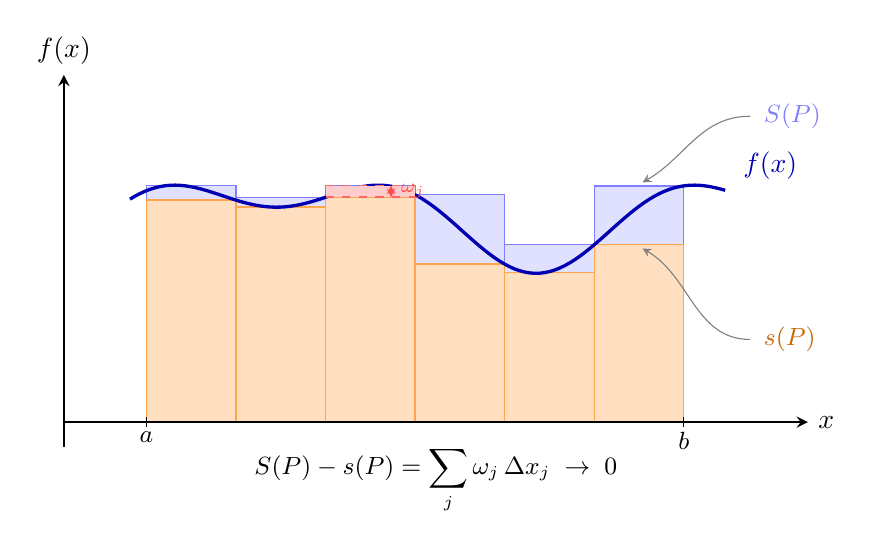
\begin{tikzpicture}[>=stealth, scale=1.05]
 
\pgfmathdeclarefunction{myfunc}{1}{%
  \pgfmathparse{0.4*sin(deg(#1-1.0))+2.5+0.3*cos(deg(2*(#1-1.0)))}%
}
 
\def\xa{1.0}
\def\xb{7.5}
\def\dx{1.083}  % (7.5-1.0)/6
 
%--- Верхние прямоугольники ---
\foreach \j in {1,2,3,4,5,6}{
  \pgfmathsetmacro{\xl}{\xa+(\j-1)*\dx}
  \pgfmathsetmacro{\xr}{\xa+\j*\dx}
  \pgfmathsetmacro{\xm}{(\xl+\xr)/2}
  \pgfmathsetmacro{\dh}{0.07}
  % approx M_j by sampling 5 points
  \pgfmathsetmacro{\va}{myfunc(\xl)}
  \pgfmathsetmacro{\vb}{myfunc(\xl+0.25*\dx)}
  \pgfmathsetmacro{\vc}{myfunc(\xm)}
  \pgfmathsetmacro{\vd}{myfunc(\xl+0.75*\dx)}
  \pgfmathsetmacro{\ve}{myfunc(\xr)}
  \pgfmathsetmacro{\Mj}{max(\va,max(\vb,max(\vc,max(\vd,\ve))))}
  \fill[blue!12] (\xl,0) rectangle (\xr,\Mj);
  \draw[blue!50, line width=0.5pt] (\xl,0) rectangle (\xr,\Mj);
}
 
%--- Нижние прямоугольники ---
\foreach \j in {1,2,3,4,5,6}{
  \pgfmathsetmacro{\xl}{\xa+(\j-1)*\dx}
  \pgfmathsetmacro{\xr}{\xa+\j*\dx}
  \pgfmathsetmacro{\xm}{(\xl+\xr)/2}
  \pgfmathsetmacro{\va}{myfunc(\xl)}
  \pgfmathsetmacro{\vb}{myfunc(\xl+0.25*\dx)}
  \pgfmathsetmacro{\vc}{myfunc(\xm)}
  \pgfmathsetmacro{\vd}{myfunc(\xl+0.75*\dx)}
  \pgfmathsetmacro{\ve}{myfunc(\xr)}
  \pgfmathsetmacro{\mj}{min(\va,min(\vb,min(\vc,min(\vd,\ve))))}
  \fill[orange!25] (\xl,0) rectangle (\xr,\mj);
  \draw[orange!70, line width=0.5pt] (\xl,0) rectangle (\xr,\mj);
}
 
%--- Штриховка зазора между S и s (только рамки верхних прямоугольников) ---
% уже видно по разным цветам
 
%--- Кривая ---
\draw[blue!70!black, very thick, domain=0.8:8.0, samples=120]
  plot (\x, {0.4*sin(deg(\x-1.0))+2.5+0.3*cos(deg(2*(\x-1.0)))});
 
%--- Оси ---
\draw[->,thick] (0,0)--(9,0) node[right]{$x$};
\draw[->,thick] (0,-0.3)--(0,4.2) node[above]{$f(x)$};
 
%--- Деления ---
\foreach \j/\lab in {0/{$a$},6/{$b$}}{
  \pgfmathsetmacro{\xp}{\xa+\j*\dx}
  \draw (\xp,0.06)--(\xp,-0.06);
  \node[below,font=\small] at (\xp,0) {\lab};
}
 
%--- Стрелки-пояснения ---
% Стрелка к верхней ступеньке
\draw[->,gray] (8.3,3.7) to[out=180,in=30] (7.0,2.90);
\node[right,font=\small,blue!50] at (8.35,3.7) {$S(P)$};
 
% Стрелка к нижней ступеньке
\draw[->,gray] (8.3,1.0) to[out=180,in=-30] (7.0,2.1);
\node[right,font=\small,orange!80!black] at (8.35,1.0) {$s(P)$};
 
%--- Обозначение «зазора» для одного столбца ---
\pgfmathsetmacro{\xLeg}{\xa+2*\dx}
\pgfmathsetmacro{\xReg}{\xa+3*\dx}
\pgfmathsetmacro{\xm}{(\xLeg+\xReg)/2}
\pgfmathsetmacro{\va}{myfunc(\xLeg)}
\pgfmathsetmacro{\vc}{myfunc(\xm)}
\pgfmathsetmacro{\ve}{myfunc(\xReg)}
\pgfmathsetmacro{\Mval}{max(\va,max(\vc,\ve))}
\pgfmathsetmacro{\mval}{min(\va,min(\vc,\ve))}
 
% штриховка зазора
\fill[red!20] (\xLeg,\mval) rectangle (\xReg,\Mval);
\draw[red!60, dashed, line width=0.6pt]
  (\xLeg,\mval) -- (\xReg,\mval)
  (\xLeg,\Mval) -- (\xReg,\Mval);
 
\draw[<->,red!70,thin]
  (\xm+0.25,\mval)--(\xm+0.25,\Mval)
  node[midway,right,font=\scriptsize]{$\omega_j$};
 
%--- Подпись ---
\node[font=\small] at (4.5,-0.7)
  {$S(P)-s(P)=\displaystyle\sum_j \omega_j\,\Delta x_j \;\to\; 0$};
 
\node[blue!70!black,font=\itshape,right] at (8.1,3.1){$f(x)$};
 
\end{tikzpicture}